\documentclass{article}
\usepackage[utf8]{inputenc}
\usepackage{indentfirst}
\usepackage[margin=1.25in]{geometry}
\usepackage{graphicx}
\usepackage{amsmath}
\usepackage{amsfonts}
\graphicspath{ {./imgs/} }

\begin{document}

\section{Logistic Regression}
This is the first post in a series that will lead to an implementation of a deep artificial neural network from scratch. 
This post will focus on the mathematical foundations behind the logistic regression. 
Throughout we will work with a training set $\mathbf{X}_{train} \in \mathbb{R}^{n\times m}$ with $n$ training samples with $m$ dimensions. We will be trying to solve a binary decision problem $\mathbf{y}_i\in\{0,1\}$. 

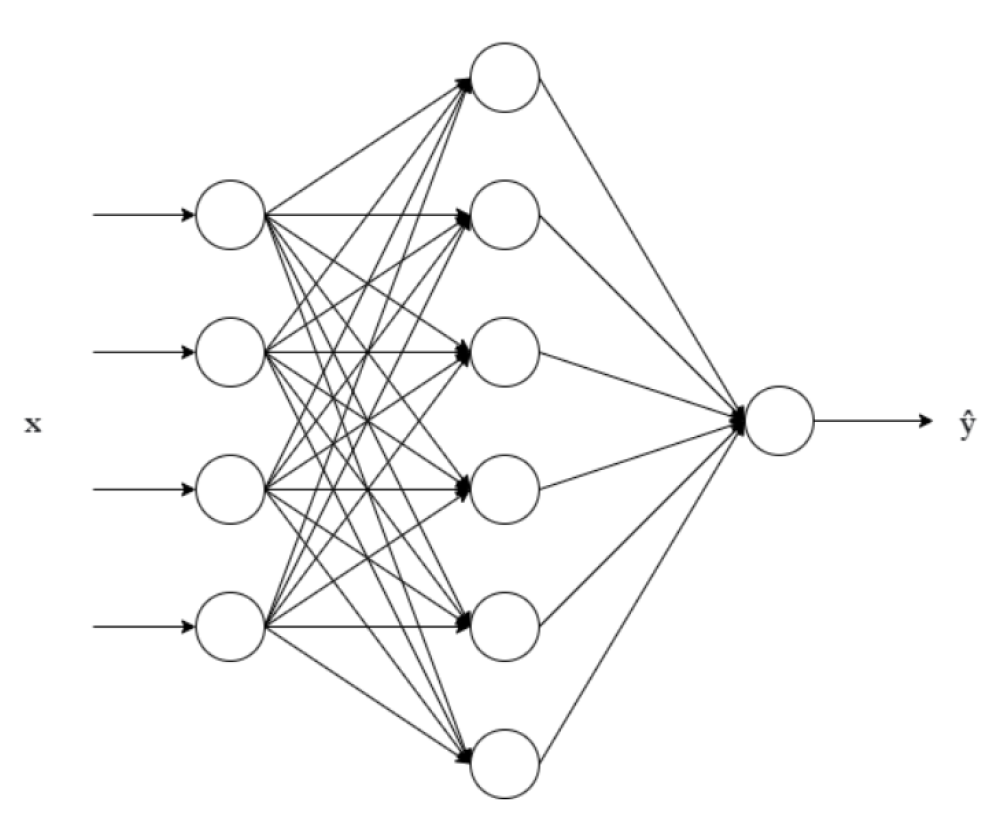
\includegraphics[scale=0.25]{210803_img1}

\subsection{Logistic Regression as a Single-Layer Neural Network}
Something tt immediately clear to me when I started machine learning was how a logistic regression could be seen as a single-layer- or a single-neuron neural network. In this context, a single-layer neural network has an input layer for the training samples, one set of weights $\mathbf{\theta}\in \mathbb{R}^{m}$, an activation function (the sigmoid in this case) and an output (layer).

The image below shows a typical representation of a fully-connected neural network with one hidden layer. The next chapter will go into more detail about these, for now you can just accept this representation as a given. 

\begin{align}
    \underset{\theta}{\text{argmax}} &\prod^N_{i=1} p(y_i|x_i, \theta) \\ 
    = &\prod^N_{i=1} g(\mathbf{\theta}^{\top} \mathbf{x}_i)^{y^i}(1-g(\mathbf{\theta}^{\top} \mathbf{x}_i))^{1-y^i}
\end{align}
\end{document}
